% Overview of how the programm is structured

\section{System Overwiev}

For monitoring the area surrounding the robot a Microsoft Kinect is used. Together with data that is received from the controller it is possible to decide whether a visible object is within a safe distance from the robot, or not. The data from each source is transformed into a joint environment.

The system consist of:
\begin{itemize}
\item A Kinect - a motion sensing input device by Microsoft.
\item Yaskawa DX100 controller - provided with a MotoPlus application.
\item Yaskawa SIA20 robot - A slim version of it predecessor IA20.
\item A Computer running the system.
\end{itemize}

\begin{figure}[H]
\begin{center}
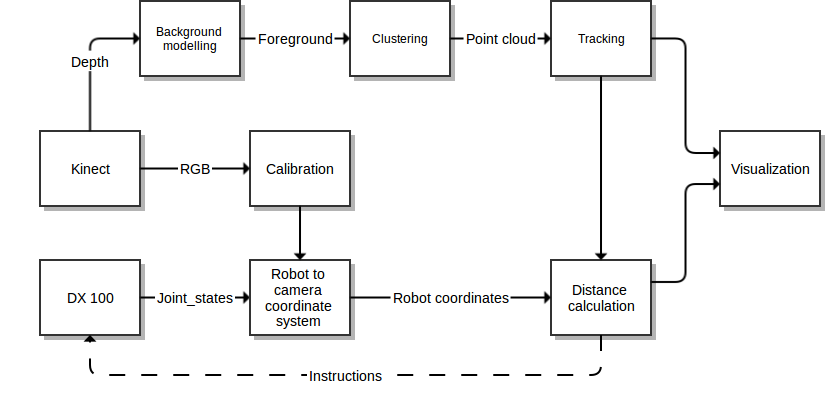
\includegraphics[width=15 cm]{flowchart}
\caption{Flowchart of system}
\label{flowchart}
\end{center}
\end{figure}




From the Kinect a depth image is provided. A background model algorithm is applied on the depth image and a foreground is obtained. The foreground only consist of moving pixels and is fairly rough. Therefore a clustering algorithm is used to extract only the relevant data. Clusters are easier to handle and much easier to track. Tracking provides a backup for what the background model might fail on. E.g. since objects might be left out from the foreground if they stay at the same place for too long.

The Kinect also provides an RGB image which makes it possible to perform calibration of the camera extrinsics using calibration patterns. Calibration algorithms are used to find transformations between different coordinates systems. This is crucial in order to measure the distance between the robot and an object.

The visualization displays a point cloud of the objects together with the robot model. Lines are used to represent the closest point pairs. The color of the line indicates in which zone the object is situated. Red emergency zone, yellow safety zone 1 and green safety zone 2.

The original idea was to send instructions to the controller. However integrating the robot with the system ended up being very time consuming. Since the topic of this project is computer vision and image processing the group decided to leave the instruction sending part out. It is possible to further develop the project to include the possibility to control the robot based on the information extracted by our system.


